\documentclass[9pt]{beamer}

%\usepackage{tikz}
\usepackage{amsmath}
\usepackage{amsfonts}
\usepackage{amssymb}
\usepackage[linesnumbered,ruled,lined]{algorithm2e}
\usepackage{color, colortbl}
\usepackage{enumerate}
\usepackage{arydshln}
\usepackage{multirow}
\usepackage{makecell}

\renewcommand{\figurename}{Fig}
\usetheme{uha}



%\theoremstyle{plain}
%  \newtheorem{theorem}{Theorem}
%  \newtheorem{lemma}{Lemma}
\newtheorem{corrolary}{Corollary}
\newtheorem{claim}{Claim}
\newtheorem{proposition}{Proposition}
\newtheorem{property}{Property}
%  \newtheorem{fact}{Fact}
%\theoremstyle{definition}
%  \newtheorem{definition}{Definition}
%  \newtheorem{example}{Example}
%\theoremstyle{remark}
\newtheorem{remark}{Remark}
\newtheorem{proviso}{Proviso}


\newcommand{\ccr}[1]{{\color{red}#1}}
\newcommand{\ccb}[1]{{\color{blue}#1}}
\newcommand{\ccp}[1]{{\color{purple}#1}}
\newcommand{\ccm}[1]{{\color{magenta}#1}}
\newcommand{\cco}[1]{{\color{orange}#1}}
\newcommand{\ccy}[1]{{\color{yellow}#1}}
\newcommand{\ccl}[1]{{\color{lime}#1}}
\newcommand{\ccc}[1]{{\color{cyan}#1}}
\newcommand{\ccg}[1]{{\color{gray}#1}}
\newcommand{\ccpk}[1]{{\color{pink}#1}}
\newcommand{\ccov}[1]{{\color{olive}#1}}



\begin{document}
	
	%%//////////////////////////////////////////////////////////////////////////////////////////////%%1
	
	\title{Matrix Decomposition}
	\subtitle{Algorithm Design}
	\author{Xinpeng Wei}
	\institute{School of Software, Shanghai Jiao Tong University}
	\date{\hspace{2em}}
	\frame{
		\titlepage
	}

	%%//////////////////////////////////////////////////////////////////////////////////////////////%%1
	
	\section{Introduction}
	
	%%//////////////////////////////////////////////////////////////////////////////////////////////%%3
	\frame{
		\frametitle{Introduction}
		\ccp{Matrix Decomposition} is a very large topic and there are lots of different decomposition for a given matrix. Such as 
		\begin{itemize}
			\item LU decomposition
			\item QR decomposition
			\item Cholesky decomposition
		\end{itemize}
		\pause
		And \ccp{LU decomposition} is useful and powerful since it can be used to solve matrix equations \ccb{$Ax=b$} fast and calculate the determinant of a square matrix.
		\[ \left[
		\begin{array}{cccc}
			a_{11} & a_{12} & \ldots & a_{1n}\\
			a_{21} & a_{22} & \ldots & a_{2n}\\
			\vdots & \vdots & \ddots & \vdots\\
			a_{n1} & a_{n2} & \ldots & a_{nn}\\
		\end{array} \right] *
		\left[\begin{array}{c}
			x_1\\
			x_2\\
			\vdots\\
			x_n
		\end{array}\right] = 
		\left[\begin{array}{c}
			b_1\\
			b_2\\
			\vdots\\
			b_n
		\end{array}\right]
		\]
	}
	\section{LU decomposition}
	\section{Definition}
	%//////////////////////////////////////////////////////////////////////////////////////////////%%4
	\frame{
		\frametitle{Definition}
		\begin{definition}{row operation}
			The row operation performed on matrix is one of the following:
			\begin{itemize}
				\item swap tow rows
				\item add one row to the other
			\end{itemize}
		\end{definition}\pause\bigskip

		\begin{definition}{Unit Lower triangular matrix}
			Given a matrix L whose order is \ccb{$n\times n$}, L is called a Unit Lower triangular matrix if and only if for any i satisfying \ccb{$1\le i\le n$}, \ccb{$L[i,i]=1$,} and for any \ccb{$i,j$} satisfying \ccb{$1\le i<j\le n$}, \ccb{$L[i, j]=0$}.
		\end{definition}\pause\bigskip

		\begin{definition}{Upper triangular matrix}
			Given a matrix L whose order is \ccb{$n\times n$}, L is called a Upper triangular matrix if and only if for any \ccb{$i,j$} satisfying \ccb{$1\le i<j\le n$}, \ccb{$L[j, i]=0$}.
		\end{definition}
	}
	\begin{frame}{Further Definition}
		\begin{definition}{LU decomposition}
			Given a matrix A whose order is \ccb{$n\times n$}, \ccb{$A=LU$} is called a LU decomposition of matrix A if and only L is a Unit Lower triangular matrix and U is an Upper triangular matrix.
		\end{definition}\pause
		\begin{figure}[h]
			\centering
			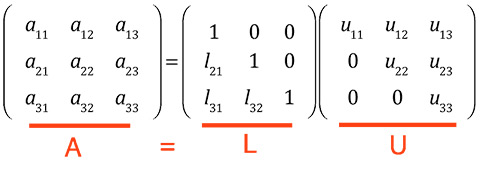
\includegraphics[width=0.65\textwidth]{figures/LU.jpeg}
		\end{figure}
	\end{frame}
	%%%//////////////////////////////////////////////////////////////////////////////////////////////%%5\\
	\subsection{Algorithms}
	\frame{
		\frametitle{Overview}
		There are lots of algorithms designed to determine the LU decomposition of a matrix.\\
		We will explore some of them step by step.\pause\bigskip
		\begin{exampleblock}{Assumption}
			In our discussion below, we assume the matrix A is fully-ranked because if not we will not get the decomposition. Also, we should note that the major task of LU decomposition is to solve \ccb{$Ax=b$} fast and sound, when A is not fully-marked there is no exact solution to the equation. So our assumption is appropriate.
		\end{exampleblock}
	}
	%%//////////////////////////////////////////////////////////////////////////////////////////////%%6
	\section{Gaussian elimination}
	\begin{frame}{Gaussian elimination}
		First we describe the algorithm\pause
		\begin{description}
			\item[step 1] Start from the first row and consider the first element of the row: if it is zero, swap the rows and get a nonzero first element. Note that this process only fails if and only if all the elements of the first column are zero thus A is not fully-ranked, which is not possible in our context.\pause
			\item[step 2] Then repeatedly do the following: for row i \ccb{$(1 < i \le n)$} , if the first element of row i is zero, just skip the row and proceed to the next row. Otherwise, we consider row i with a nonzero first element \ccb{$X_{i}$}, then add row 1 multiply \ccb{$-X_{i}/P_{1} $} to row i, \ccb{$P_{1}$} is the first element of row 1,we eliminate the first element of row i to zero.\pause
			\item[step 3] just continue the loop until we finally get an Upper triangular matrix.
		\end{description}
	\end{frame}

	\begin{frame}{Gaussian elimination}
		\begin{lemma}
			swap two rows is equivalent to left multiplication a identity matrix with row i and j swapped.
		\end{lemma}\pause
		\ccm{\em Proof.}
The P satisfies following properties
		\begin{enumerate}
			\item for $1\le k\le n,k \neq i,j$, $P[k,k]=1$
			\item $P[j,i]=P[i,j]=1$
			\item for all other pair $(i,j)$, $P[i, j] = 0$
		\end{enumerate}
		Now it's easy to confirm that $A_t=PA$ is the same as A with row i and j swapped.
	\end{frame}

	\begin{frame}{Gaussian elimination}
		\begin{lemma}
			add one row to the other is equivalent to left multiplication a identity matrix with row i added to row j.
		\end{lemma}\pause
		\ccm{\em Proof.} The P satisfies following properties
		\begin{enumerate}
			\item for $1 \le k \le n$, $P[k,k]=1$.
			\item $P[j,i]=1$.
			\item for all other pair $(i,j)$,$P[i,j]=0$.
		\end{enumerate}
		The same as last lemma, we can do the matrix multiplication and confirm that \ccb{$A_t=PA$} is the same as A with row i added to row j.
	\end{frame}

	\begin{frame}{Gaussian elimination}
		\begin{block}{Theorem 1}
			the row operations performed on matrix are equivalent to pre-multiply a certain matrix P.
		\end{block}\pause
		\ccm{\em Proof.} We finish the proof with two kinds of row operations defined above.
	\end{frame}

	\begin{frame}{Gaussian elimination}
		\begin{block}{Theorem 2}
			the product of two Unit lower triangular matrix is a Unit lower triangular matrix.
		\end{block}\pause
		\ccm{\em Proof.} let A and B are Unit lower triangular matrix. We compute the product of A and B, let C = AB.
		\begin{enumerate}
			\item we compute all diagonal elements of C.
			C[i,i]=$\Sigma_{k=1}^{k=n}A[i,k]B[k,i]$. Note that A,B are Unit lower triangular matrix, so for $1 \le k < i$, $B[k,i] = 0$ and for $i < k \le n$, $A[i,k] = 0$, $B[i,i]=1$ and $A[i,i]= 1$. Use the three facts above, we get C[i,i]=1.
			\item we now prove for $1 \le i < j \le n$, C[i,j]=0.
			C[i,j]=$\Sigma_{k=1}^{k=n}A[i,k]B[k,j]$, since for $1 \le k < j$, B[k,j] = 0 and for $i < k \le n$, A [i,k] = 0, So $1 \le k < j$, A[i,k]B[k,j] = 0 and for $i < k \le n$, A [i,k]B[k,j] = 0, we get C[i,j] = 0
		\end{enumerate}
	\end{frame}

	\begin{frame}{Gaussian elimination}
		Based on the theorems above, we first do the row swap such that during the elimination, the diagonal element of A is nonzero. as we have proved this leads to \ccb{$PA$}, then we do the elimination by adding one row to the other, by the  5, this can be done by a series of pre-multiply: \ccb{$E_{1}E_{2}...E_{n}PA=U$}, and by Lemma 6, we get \ccb{$PA=E_{n}^{-1}...E_{2}^{-1}E_{1}^{-1}U=LU$}, note that the redundant P do not interfere with our goal because in practice we just first do the swap.
	\end{frame}

	\begin{frame}{Complexity}
		\begin{theorem}
			The time complexity of Gaussian Elimination is \ccb{$O(n^3)$}
		\end{theorem}\pause\bigskip
		\ccm{\em Proof.} It's obvious since we eliminate every column use \ccb{$O(n^2)$} multiplication and addition and there are n rows.
	\end{frame}

	\begin{frame}{In practice}
		\begin{itemize}
			\item The complexity(\ccb{$O(n^3)$}) in real world is not acceptable as n is usually incredibly large, typically $10^5$.\pause\bigskip
			\item The conditional number of the procedure above is very large which means the solution is susceptible to inaccuracy of the data caused by float point number operation.
		\end{itemize}
	\end{frame}
	%%//////////////////////////////////////////////////////////////////////////////////////////////%%7
	\section{Left Looking elimination}
	\begin{frame}{Left Looking Elimination}
		Let's derive a left looking version of Gaussian elimination.\\ \pause
		We can further extend this approach to our real world practice.\\ \pause\bigskip
		\begin{figure}[h]
			\centering
			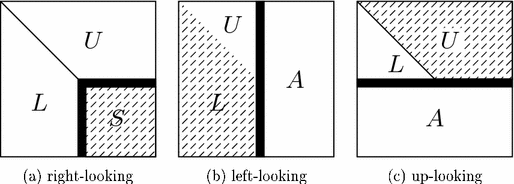
\includegraphics[width=0.65\textwidth]{figures/left_LU.png}
			\caption{Three main *-looking LU}
		\end{figure}
	\end{frame}
	\begin{frame}{Declaration}
		Given an input matrix A with order of \ccb{$n\times n$} can be represented as a product of two triangular matrices L and U. We write A as follow:
		\[
			\left( \begin{array}{ccc} A_{11} & \pmb{\alpha_{12}}  & A_{13}\\ \pmb{\alpha_{21}} & a_{22}  & \pmb{\alpha_{23}}\\  A_{31} & \pmb{\alpha_{32}}  & A_{33}\\ \end{array} \right)  = \left( \begin{array}{ccc} L_{11} & 0  & 0\\ \pmb{l_{21}} & 1  & 0\\  L_{31} & \pmb{l_{32}}  & L_{33}\\ \end{array} \right) \times \left( \begin{array}{ccc} U_{11} & \pmb{u_{12}}  & U_{13}\\ 0 & u_{22}  & \pmb{u_{23}}\\  0 & 0  & U_{33}\\ \end{array} \right)
		\]
	where \ccb{$A_{ij}$} is a block, \ccb{$\pmb{\alpha_{ij}}$} is a vector and \ccb{$a_{ij}$} is a scalar. The dimensions of different elements in the matrices are as follows:
	\end{frame}
	\begin{frame}{Declaration}
		\[
		\left( \begin{array}{ccc} A_{11} & \pmb{\alpha_{12}}  & A_{13}\\ \pmb{\alpha_{21}} & a_{22}  & \pmb{\alpha_{23}}\\  A_{31} & \pmb{\alpha_{32}}  & A_{33}\\ \end{array} \right)  = \left( \begin{array}{ccc} L_{11} & 0  & 0\\ \pmb{l_{21}} & 1  & 0\\  L_{31} & \pmb{l_{32}}  & L_{33}\\ \end{array} \right) \times \left( \begin{array}{ccc} U_{11} & \pmb{u_{12}}  & U_{13}\\ 0 & u_{22}  & \pmb{u_{23}}\\  0 & 0  & U_{33}\\ \end{array} \right)
		\]
		\begin{itemize}
			\item $A_{11},L_{11},U_{11}$ are $k \times k$ blocks
			\item $\pmb{\alpha_{12}}, \pmb{u_{12}}$ are $k \times 1$ vectors
			\item $A_{13},U_{13}$ are $k\times n-(k+1)$ blocks
			\item $\pmb{\alpha_{21}},\pmb{l_{21}}$ are $1 \times k$ row vectors
			\item $a_{22},u_{22}$ are scalars
			\item $\pmb{\alpha_{23}},\pmb{u_{23}}$ are $1\times n-(k+1)$ row vectors
			\item $A_{31},L_{31}$ are $n-(k+1) \times k$ blocks
			\item $\pmb{\alpha_{32}},\pmb{l_{32}} $ are $n-(k+1)\times 1$vectors
			\item $A_{33},L_{33},U_{33}$ are $n-(k+1)\times n-(k+1)$ blocks
		\end{itemize}
	\end{frame}

	\begin{frame}{Solve}
		\[
		\left( \begin{array}{ccc} A_{11} & \pmb{\alpha_{12}}  & A_{13}\\ \pmb{\alpha_{21}} & a_{22}  & \pmb{\alpha_{23}}\\  A_{31} & \pmb{\alpha_{32}}  & A_{33}\\ \end{array} \right)  = \left( \begin{array}{ccc} L_{11} & 0  & 0\\ \pmb{l_{21}} & 1  & 0\\  L_{31} & \pmb{l_{32}}  & L_{33}\\ \end{array} \right) \times \left( \begin{array}{ccc} U_{11} & \pmb{u_{12}}  & U_{13}\\ 0 & u_{22}  & \pmb{u_{23}}\\  0 & 0  & U_{33}\\ \end{array} \right)
		\]
		Now, we calculate the equation and get following equations:
		\begin{itemize}
			\item $L_{11}\times U_{11} = A_{11}$
			\item $L_{11}\times \pmb{u_{12}} = \pmb{\alpha_{12}}$
			\item $L_{11}\times U_{13} = A_{13}$
			\item $\pmb{l_{21}} \times U_{11} = \pmb{\alpha_{21}}$
			\item $\pmb{l_{21}} \times  \pmb{u_{12}} + u_{22} = a_{22}$
			\item $\pmb{l_{21}} \times U_{13} + \pmb{u_{23}} = \pmb{\alpha_{23}}$
			\item $L_{31}\times U_{11} = A_{31}$
			\item $L_{31}\times \pmb{u_{12}} +\pmb{l_{32}}\times u_{22} = \pmb{\alpha_{32}}$
		\end{itemize}
	\end{frame}

	\begin{frame}{Clarification}
		The method is called \ccp{Left-looking elimination} because if computes the \ccb{$k^{th}$} column of L and U using their $1,2...k-1$ columns.\\ \pause\bigskip
		Suppose we already know the first \ccb{$k-1$} columns. We can extract the parts interesing us and get the following equation:\bigskip
		\[
			\left( \begin{array}{ccc} L_{11} & 0  & 0\\ \pmb{l_{21}} & 1  & 0\\  L_{31} & 0  & 1\\ \end{array} \right) \times\left( \begin{array}{ccc} \pmb{u_{12}}   \\ u_{22}   \\  \pmb{l_{32}}\times u_{22} \\ \end{array} \right) = \left( \begin{array}{ccc}  \pmb{\alpha_{12}} \\ a_{22}\\ \pmb{\alpha_{32}}  \\ \end{array} \right)
		\]
	\end{frame}

	\begin{frame}{Compute}
		\[
		\left( \begin{array}{ccc} L_{11} & 0  & 0\\ \pmb{l_{21}} & 1  & 0\\  L_{31} & 0  & 1\\ \end{array} \right) \times\left( \begin{array}{ccc} \pmb{u_{12}}   \\ u_{22}   \\  \pmb{l_{32}}\times u_{22} \\ \end{array} \right) = \left( \begin{array}{ccc}  \pmb{\alpha_{12}} \\ a_{22}\\ \pmb{\alpha_{32}}  \\ \end{array} \right)
		\]\bigskip
		
		\ccb{$\pmb{u_{12}},u_{22},\pmb{l_{32}}$} is all what we need to get the \ccb{$k^{th}$} column of L and U, and it is clear how to get them:
		\begin{itemize}
			\item first compute $L_{11}\times \pmb{u_{12}} = \pmb{\alpha_{12}}$, we get $\pmb{u_{12}}$
			\item then compute $  u_{22} = a_{22} - \pmb{l_{21}} \times  \pmb{u_{12}}$, we get $u_{22}$
			\item finally compute  $ \pmb{l_{32}}  =\frac{1}{u_{22}}( \pmb{\alpha_{32}} - L_{31}\times \pmb{u_{12}})$,we get $ \pmb{l_{32}}$
		\end{itemize}\pause
		step 2 and 3 are easy since they just involve multiplication and addition.\\
		How to compute \ccb{$u_{12}$}?
	\end{frame}

	\begin{frame}{Compute $u_{12}$}
		Note \ccb{$L_{11}$} is the upper \ccb{$k\times k$} blocks of Unit lower triangular L, so \ccb{$L_{11}$} is also Unit lower triangular. Hence we can derive a simple algorithm.
		\begin{exampleblock}{}
			\begin{algorithm}[H]
			$x\gets b$\;
			\For{$i=1$ \KwTo $n$}
			{
				\If{$x(i)\neq 0$}{
					\For{$j=i+1$ \KwTo $n$}{
						$x(j)=x(j)-L(j,i)*x(i)$
					}
				}
			}
			\end{algorithm}
		\end{exampleblock}
	\end{frame}

	\begin{frame}{Complexity}
		\begin{theorem}
			The time complexity of Left-Looking Elimination is \ccb{$O(n^2)$}
		\end{theorem}\pause\bigskip
		\ccm{\em Proof.} Every time we compute \ccb{$\pmb{u_{12}}$}, we use \ccb{$O(n+\text{number of multiplications})$}\\
		And we have n iterations. So it seems likely to be \ccb{$O(n^3)$}, but the vector addition can be improved to nearly \ccb{$O(1)$}, thus we can think this approach can achieve at most \ccb{$O(n^2)$}.\pause
		\begin{alertblock}{In practice}
			Although far more better than the Gauss-Elimination, it is not practical to put into use in industry as well due to quadratic complexity.
		\end{alertblock}
	\end{frame}

	\section{A Practival method: G-P Algotithm}
	\begin{frame}{Brief}
		\ccp{Gauss Elimination} and \ccp{Left-Looking Elimination} are not efficient in large scale input.\\
		But in real practice, a certain kind of problems share some common characteristics.\\ \pause\bigskip
		\ccp{Gilbert Peierls Algorithm} is one of the algorithms that exploit these characteristics.
		Almost all further improvement algorithms are based on the idea proposed by Gilbert Peierls Algorithm.
		\begin{figure}[h]
			\centering
			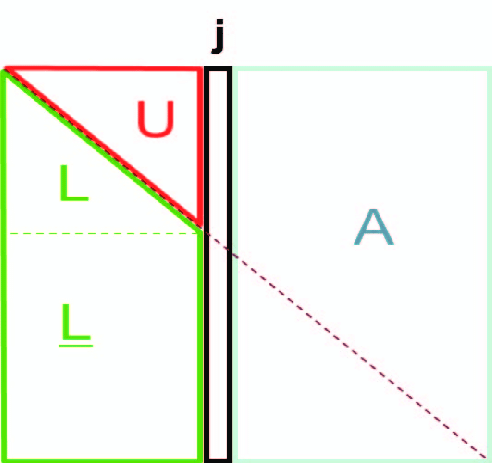
\includegraphics[width=0.3\textwidth]{figures/Gilbert-Peierls-LU.png}
			\caption{Gilbert Peierls LU}
		\end{figure}
	\end{frame}

	\begin{frame}{sparse matrix}
		\begin{definition}{sparse matrix}
			A matrix is called sparse if the nonzero elements is very few. In practice, we usually call a matrix sparse if it has \ccb{$O(n)$}
		\end{definition}\pause
	For sparse matrixs, we usually them using the column compressed form and it only takes \ccb{$O(n)$} space.
	\end{frame}

	\begin{frame}{Column compressed form}
		\begin{definition}{column compressed form}
			A column compressed form of a matrix consists of three vectors: \ccb{$A_{p},A_{i},A_{x}$}
			\begin{table}[h]
				\centering
				\begin{tabular}{c|c}
					\hline
					column  & definition\\ \hline\hline
					$A_{x}$ & \makecell[c]{contains all the nonzero elements of A\\ from column 1 to column n} \\ \hline
					$A_{i}$ & \makecell[c]{contains all the nonzero elements column index\\ from column 1 to column n} \\ \hline
					$A_{p}$ &\makecell[c]{contains all the ending index of a given column in $A_{i}$\\ except the first element is always 0} \\ \hline
				\end{tabular}
			\end{table}
		\end{definition}
	\end{frame}

	\begin{frame}{Quiz}
			Given matrix
			\[\left(
			\begin{array}{ccc}
				5 & 0 & 0\\
				4 & 2 & 0\\
				3 & 1 & 8\\
			\end{array}
			\right)\]
			What's the corresponding column compressed format ? \pause
			\begin{table}[h]
				\centering
				\begin{tabular}{c|c}
					\hline
					column  & value    \\ \hline\hline
					$A_{x}$ & $5,4,3,2,1,8$     \\
					$A_{i}$ & $0,1,2,1,2,2$ \\
					$A_{p}$ & $0,3,5,6$     \\ \hline
				\end{tabular}
			\end{table}
	\end{frame}

	\section{Gilbert Peierls Algorithm}
	\begin{frame}
		\begin{block}{Aim}
			Decomposition arbitary non singular sparse matrix \ccb{$A$} as \ccb{$PA=LU$} in time proportion to the flop count of the L and U.
		\end{block}\pause
		\begin{definition}{flops(LU)}
			The symbol flops(LU) is the number of nonzero multiplications performed when multiplying two matrices L and U.
		\end{definition}\pause
		\centering
		\cco{We analysis the complexity the algorithm based on the flops(LU).}
	\end{frame}

	\begin{frame}{Symbolic analysis}
. The time complexity is \ccb{$O(n+\text{number of flops performed})$}, we can remove the \ccb{$O(n)$} term using the follow one.\pause
		\begin{exampleblock}{}
			\begin{algorithm}[H]
				$x\gets b$\;
				\For{all $i$ satisfying $x(i)\neq 0$}
				{
					\For{$j=i+1$ \KwTo $n$}{
						$x(j)=x(j)-L(j,i)*x(i)$
					}
				}
			\end{algorithm}
		\end{exampleblock}\pause
		\cco{Improvement: This would reduce the \ccb{$O(n)$} to \ccb{$O(\eta(x))$}}\\ \pause
		\ccr{Q}: how to recognize nonzero pattern of $x$ before we compute $x$ itself?
	\end{frame}

	\begin{frame}{Symbolic analysis}
		\begin{theorem}
			Let \ccb{$G = G(L_k)$} be the directed graph of L with \ccb{$k-1$} vertices representing the already computed \ccb{$k-1$} columns. \ccb{$G(L_k)$} has an edge \ccb{$j \rightarrow i$} if and only if \ccb{$l_{ij} \neq 0$}. Let \ccb{$\beta = \{ i | b_i \ne 0 \}$} and \ccb{$X = \{ i | x_i \ne 0 \}$}, Now the elements of X is given by
			\[
				X = Reach_{G(L)}(\beta)
			\]
		\end{theorem}\pause\bigskip
		\ccm{\em Proof.} The proof is very tricky so we don't cover it here.
	\end{frame}
	
	\begin{frame}{Symbolic analysis}
		\begin{theorem}
			Let \ccb{$G = G(L_k)$} be the directed graph of L with \ccb{$k-1$} vertices representing the already computed \ccb{$k-1$} columns. \ccb{$G(L_k)$} has an edge \ccb{$j \rightarrow i$} if and only if \ccb{$l_{ij} \neq 0$}. Let $\beta = \{ i | b_i \ne 0 \}$ and \ccb{$X = \{ i | x_i \ne 0 \}$}, Now the elements of X is given by
			\[
			X = Reach_{G(L)}(\beta)
			\]
		\end{theorem}
		\cco{Observation}: The nonzero pattern of \ccb{$X$} is computed by determining the vertices reachable from the vertices of the set $\beta$.\\ \pause
		\ccr{Solution}: So we can just use a depth first search from the vertives of the set $\beta$ during which we also can get a topological order of X which is useful for eliminating unknowns in the next step.
	\end{frame}
	
	\begin{frame}{Numerical Factorization}
		\ccp{Numerical Factorization} consists of solving for each column of \ccb{$L$} and \ccb{$U$}.\\ \pause\bigskip
		We usually solve the equation in increasing order of the row index.\\ \pause
		But row indeces computed from DFS aren't in right order and sorting is really time-cosuming.\\ \pause\bigskip
		\cco{Loose}: We use topological order of the row indices instead.\\ \pause\bigskip
		\ccm{\em Proof.} Once all the unknowns \ccb{$x_j$} of which it's dependent are computed, an unknown \ccb{$x_i$} can be computed.
	\end{frame}

	\begin{frame}{Complete picture}
		We finally got the algorithm:
		\begin{exampleblock}{}
			\begin{algorithm}[H]
				$L \gets I$\;
				\For{$i=1$ \KwTo $n$}
				{
					$X\gets L\setminus k_{th}$ column of $A$\;
					\For{$j=1$ \KwTo $i$}{
						$U(j,k) = x(j)$
					}
					\For{$j=k$ \KwTo n}{
						$L(j,k)=x(j)/U(k,k)$
					}
				}
			\end{algorithm}
		\end{exampleblock}
		\ccb{$x = L\backslash b$} in the above algorithm denotes the solution of: \ccb{$Lx =b$}. In this case, b is the \ccb{$k^{th}$} column of A.\pause
	\end{frame}

	\begin{frame}{Complexity}
		\begin{theorem}
			The time complexity of the algorithm is \ccb{$O(\eta(A)+flops(LU))$}. 
		\end{theorem}
		\ccb{$\eta(A)$} is the number of nonzeros in the matrix A and \ccb{$flops(LU)$} is the flop count of the product of the matrices L and U. We also do a depth first search, it costs nearly \ccb{$O(n)$}.\\ \pause
		\cco{Claim}: \ccb{$flops(LU)$} is less then the nonzero element in L or U.\\ \pause\bigskip
		\ccr{Q}: Won't it reach \ccb{$O(n^2)$}?\\ \pause
		\cco{A}: In practice, it works really fast, slightly bigger than \ccb{$O(n)$}.\\ \pause\bigskip
		So the \ccb{$flops(LU)$} dominants and we can assume it's \ccb{$O(flops(LU))$}.
	\end{frame}

	\begin{frame}{Conclusion}
		The Gilbert Peierls Algorithm is the base decomposition algorithm for scientific computing package such as Matlab, numpy, OpenBLAS and SuiteSparse.
		\begin{figure}[H]
			\centering
			\begin{minipage}[ht]{0.5\linewidth}   
				\centering   
				
\includegraphics[width=0.8\textwidth]{figures/numpy.jpeg}
			\end{minipage}
			\begin{minipage}[ht]{0.5\linewidth} % 如果一行放2个图,用0.5,如果3个图,用0.33
				\centering
				
\includegraphics[width=0.8\textwidth]{figures/matlab.jpeg}
			\end{minipage}
			\begin{minipage}[ht]{0.4\linewidth} % 如果一行放2个图,用0.5,如果3个图,用0.33
				\centering
				
\includegraphics[width=0.8\textwidth]{figures/SuiteSparse.jpg}
			\end{minipage}
		\end{figure}
	\end{frame}
	
	\begin{frame}{Numpy}
		We can see KLU's usage in numpy's main repository on \href{https://github.com/numpy/numpy}{GitHub}.
		\begin{figure}[H]
			\centering
			\begin{minipage}[ht]{0.4\linewidth} % 如果一行放2个图,用0.5,如果3个图,用0.33
				\centering
				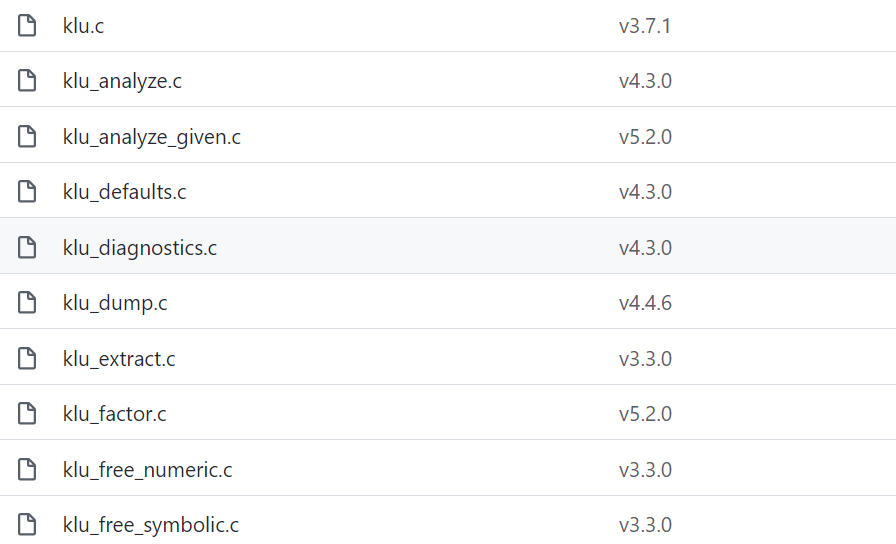
\includegraphics[width=1\textwidth]{figures/numpy1.jpg}
			\end{minipage}
			\begin{minipage}[ht]{0.4\linewidth} % 如果一行放2个图,用0.5,如果3个图,用0.33
				\centering
				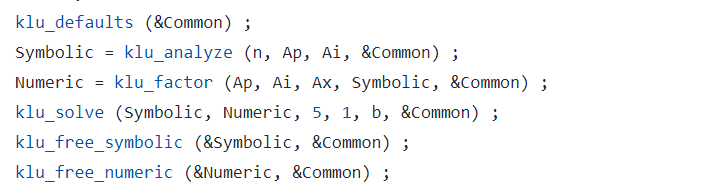
\includegraphics[width=1.2\textwidth]{figures/numpy2.jpg}
			\end{minipage}
		\end{figure}
	\end{frame}

\end{document}